\chapter{Mô hình hóa chức năng}

\section{Tác nhân (Actors)}

\begin{table}[h]
\centering
\caption{Danh sách tác nhân của hệ thống}
\label{tab:actors}
\begin{tabular}{P{3.6cm}P{4.2cm}P{7.2cm}}
\toprule
\textbf{Tác nhân} & \textbf{Vai trò hệ thống} & \textbf{Mô tả} \\
\midrule
Nhân viên đơn vị sử dụng & DON\_VI & Khai báo, báo sự cố, tự khắc phục sự cố nhỏ, cập nhật hồ sơ của thiết bị thuộc đơn vị mình \\
Văn phòng Cục & VAN\_PHONG\_CUC & Quản lý danh mục tổng, lập kế hoạch, xem xét sự cố, lập phương án, lập biên bản nghiệm thu, quản trị người dùng/nhà thầu \\
Lãnh đạo Cục & LANH\_DAO\_CUC & Phê duyệt/từ chối kế hoạch và phương án sửa chữa \\
Ban QMS & QMS & Xem báo cáo, theo dõi nhật ký thao tác, giám sát tuân thủ \\
Nhà thầu ngoài & NHA\_THAU & Tham gia ký biên bản nghiệm thu (mở rộng) \\
Bộ nhắc lịch & (job hệ thống) & Tác nhân phi con người: chạy 07:00 hằng ngày, gửi thông báo hạng mục đến hạn \\
\bottomrule
\end{tabular}
\end{table}

\section{Danh sách use case}

\begin{longtable}{P{1.8cm}P{9.4cm}P{4.2cm}}
\caption{Danh mục use case và truy vết về quy trình gốc}\label{tab:uc-list}\\
\toprule
\textbf{Mã} & \textbf{Use case} & \textbf{Tác nhân chính} \\
\midrule
\endfirsthead
\toprule
\textbf{Mã} & \textbf{Use case} & \textbf{Tác nhân} \\
\midrule
\endhead
UC-01 & Đăng nhập hệ thống & Tất cả \\
UC-02 & Quản lý danh mục trang thiết bị (BM/01) & Văn phòng Cục \\
UC-03 & Cập nhật hồ sơ trang thiết bị (BM/02) & Văn phòng Cục, Đơn vị \\
UC-04 & Báo sự cố & Đơn vị, Văn phòng Cục \\
UC-05 & Xem xét, xác định nguyên nhân sự cố & Văn phòng Cục \\
UC-06 & Tự khắc phục sự cố nhỏ & Đơn vị (\textit{extend} UC-05 khi sự cố nhỏ) \\
UC-07 & Lập phương án sửa chữa / thuê ngoài & Văn phòng Cục (\textit{include} UC-08) \\
UC-08 & Trình phê duyệt & (dùng chung) \\
UC-09 & Phê duyệt phương án sửa chữa & Lãnh đạo Cục \\
UC-10 & Lập kế hoạch bảo dưỡng, thay thế năm (BM/03) & Văn phòng Cục (\textit{include} UC-08) \\
UC-11 & Phê duyệt kế hoạch bảo dưỡng năm & Lãnh đạo Cục \\
UC-12 & Thực hiện bảo dưỡng / sửa chữa & Văn phòng Cục, Đơn vị, Nhà thầu \\
UC-13 & Lập biên bản nghiệm thu (BM/04) & Văn phòng Cục (\textit{extend} UC-12 khi thuê ngoài) \\
UC-14 & Xem báo cáo \& thống kê & Ban QMS, Lãnh đạo Cục, Văn phòng Cục \\
UC-15 & Nhắc lịch bảo dưỡng định kỳ & Bộ nhắc lịch \\
\bottomrule
\end{longtable}

Quan hệ \texttt{<<include>>} và \texttt{<<extend>>}:
\begin{itemize}
  \item UC-07 và UC-10 \texttt{<<include>>} UC-08 (Trình phê duyệt) — mọi tài liệu trình duyệt dùng chung một cơ chế.
  \item UC-06 \texttt{<<extend>>} UC-05 với điều kiện \{sự cố nhỏ\} — đúng rẽ nhánh 6.2.3b.
  \item UC-13 \texttt{<<extend>>} UC-12 với điều kiện \{thuê ngoài\} — nghiệm thu chỉ bắt buộc khi thuê ngoài (mục 6.2.5).
  \item UC-13 \texttt{<<extend>>} UC-03 với điều kiện \{sau nghiệm thu/khắc phục\} — cập nhật hồ sơ là bước kết thúc.
\end{itemize}

\begin{figure}[h]
\centering
% Nguồn: docs/diagrams/01-use-case.drawio — xuất PNG đặt vào figures/
\IfFileExists{figures/use-case.png}{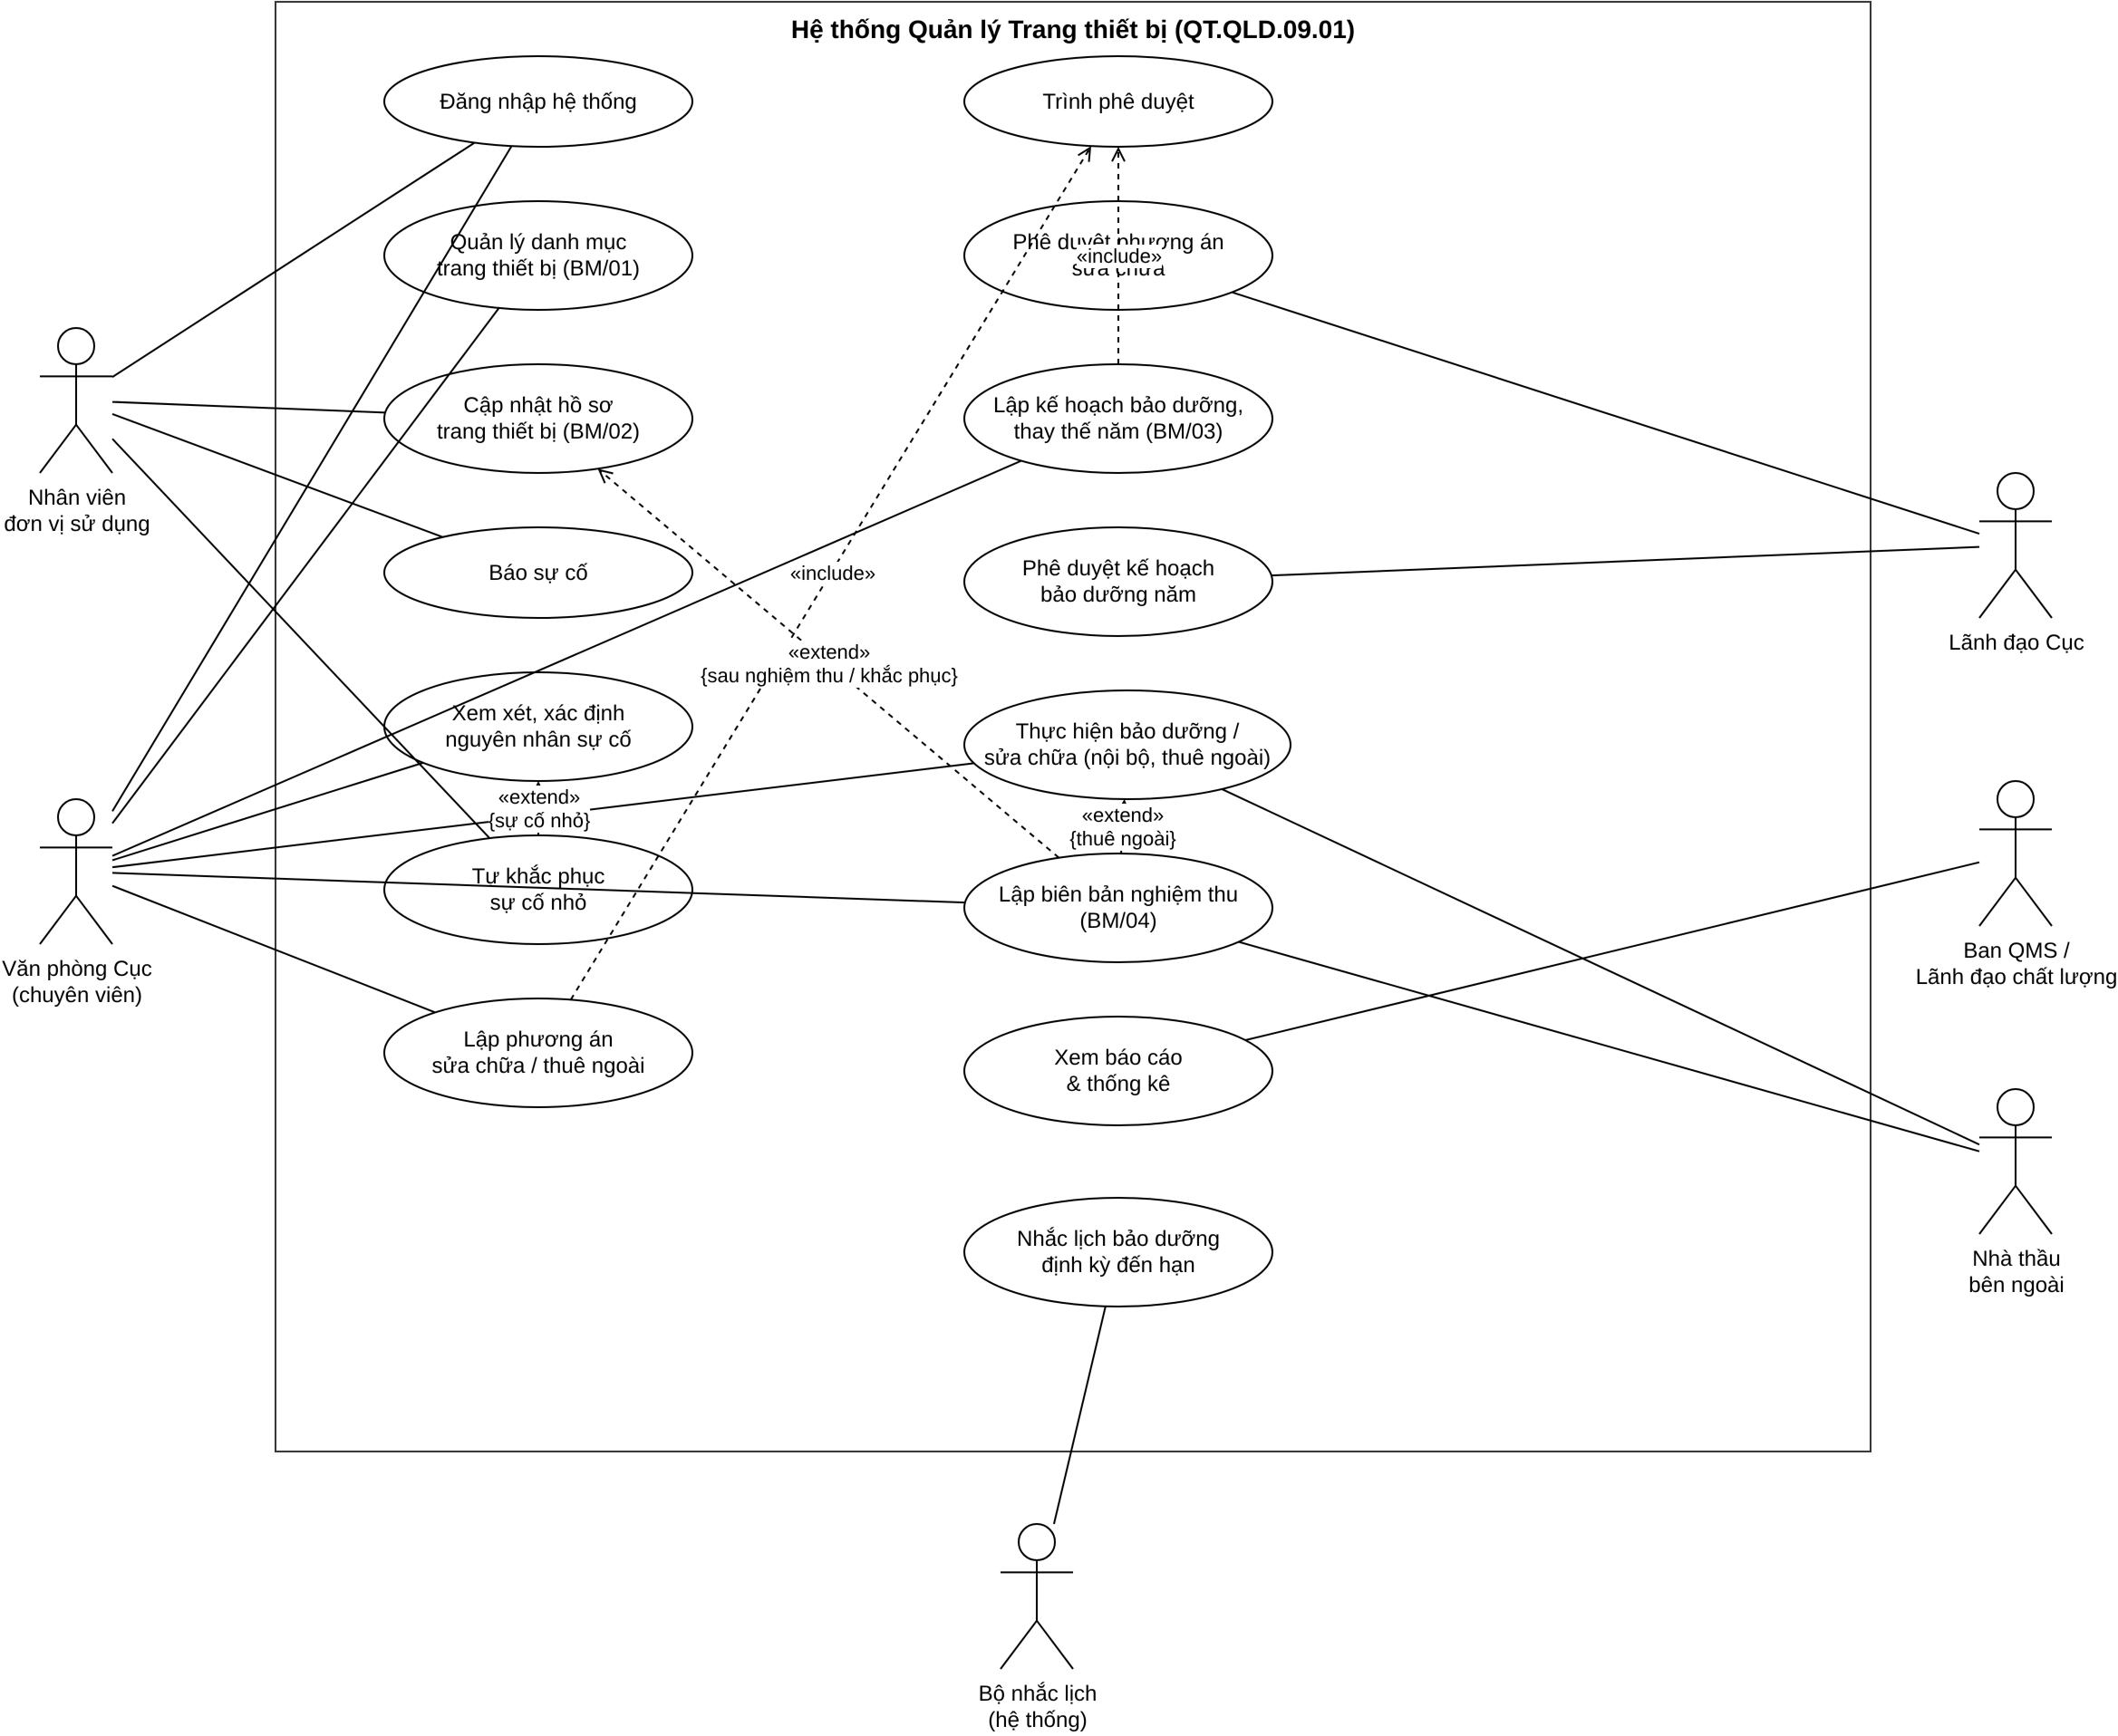
\includegraphics[width=\textwidth]{figures/use-case.png}}{\fbox{\parbox{0.9\textwidth}{\centering Sơ đồ use case (xem file \texttt{docs/diagrams/01-use-case.drawio} — mở bằng draw.io)}}}
\caption{Sơ đồ use case tổng quát của hệ thống}
\label{fig:usecase}
\end{figure}

\section{Đặc tả use case chính}

\begin{table}[h]
\centering
\caption{Đặc tả UC-04: Báo sự cố}
\label{tab:uc04}
\begin{tabular}{P{3.2cm}P{11.8cm}}
\toprule
\textbf{Use case} & UC-04 — Báo sự cố \\
\textbf{Tác nhân} & Nhân viên đơn vị sử dụng (chính); Văn phòng Cục (bổ sung) \\
\textbf{Tiền điều kiện} & Đã đăng nhập (UC-01); thiết bị nằm trong danh mục và thuộc đơn vị \\
\textbf{Hậu điều kiện} & Sự cố tạo mới với trạng thái ``Mới''; thiết bị chuyển ``Sự cố''; Văn phòng Cục nhận thông báo \\
\midrule
\textbf{Luồng chính} & 1. Đơn vị chọn ``Báo sự cố''. \; 2. Hệ thống hiển thị danh sách thiết bị của đơn vị. \; 3. Đơn vị chọn thiết bị, chọn mức độ ước lượng (nhỏ/nguy cơ/lớn), nhập mô tả. \; 4. Hệ thống kiểm tra dữ liệu hợp lệ. \; 5. Hệ thống sinh mã sự cố (SC-<năm>-<số thứ tự>), lưu với trạng thái ``Mới'', chuyển thiết bị sang ``Sự cố'', gửi thông báo cho Văn phòng Cục, ghi audit log. \; 6. Hệ thống hiển thị mã sự cố cho đơn vị. \\
\textbf{Luồng thay thế} & 4a. Thiếu thiết bị/mô tả: hiển thị lỗi, quay lại bước 3. \newline 5a. Thiết bị không tồn tại hoặc không thuộc đơn vị: báo lỗi 404/403. \\
\bottomrule
\end{tabular}
\end{table}

\begin{table}[h]
\centering
\caption{Đặc tả UC-05 + UC-06: Xem xét nguyên nhân và tự khắc phục}
\label{tab:uc05}
\begin{tabular}{P{3.2cm}P{11.8cm}}
\toprule
\textbf{Use case} & UC-05 — Xem xét, xác định nguyên nhân (gồm UC-06) \\
\textbf{Tác nhân} & Văn phòng Cục (chính), Đơn vị (trong UC-06) \\
\textbf{Tiền điều kiện} & Tồn tại sự cố trạng thái ``Mới'' \\
\textbf{Hậu điều kiện} & Nếu [nhỏ]: sự cố ở ``Đang xem xét'' với phân loại ``Tự khắc phục''; nếu [lớn]: ``Chờ phê duyệt'' chờ lập phương án \\
\midrule
\textbf{Luồng chính} & 1. Văn phòng Cục mở danh sách sự cố ``Mới''. \; 2. Chọn ``Xem xét'', nhập mức độ, nguyên nhân. \; 3. Chọn phân loại: \emph{Tự khắc phục} / \emph{Nội bộ} / \emph{Thuê ngoài}. \; 4. Hệ thống cập nhật trạng thái: [tự khắc phục] $\rightarrow$ ``Đang xem xét'' và thông báo cho đơn vị; [khác] $\rightarrow$ ``Chờ phê duyệt''. \; 5. Ghi audit log. \\
\textbf{UC-06} & 6. Đơn vị mở ``Sự cố của đơn vị'', chọn ``Tự khắc phục'', nhập nội dung khắc phục. \; 7. Hệ thống \textbf{tự động ghi một bản ghi vào hồ sơ thiết bị (BM/02)}, đóng sự cố, trả thiết bị về ``Hoạt động''. \; \textbf{Không có bước phê duyệt} — đúng mục 6.2.3b. \\
\textbf{Luồng thay thế} & 7a. Thiếu nội dung khắc phục: báo lỗi, giữ trạng thái. \newline 2a. Sự cố không ở trạng thái ``Mới'': từ chối (409). \\
\bottomrule
\end{tabular}
\end{table}

\begin{table}[h]
\centering
\caption{Đặc tả UC-10 + UC-11: Lập và phê duyệt kế hoạch bảo dưỡng năm}
\label{tab:uc10}
\begin{tabular}{P{3.2cm}P{11.8cm}}
\toprule
\textbf{Use case} & UC-10 — Lập kế hoạch bảo dưỡng, thay thế năm (gồm UC-11) \\
\textbf{Tác nhân} & Văn phòng Cục (chính); Lãnh đạo Cục (UC-11) \\
\textbf{Tiền điều kiện} & Đã có danh mục thiết bị; chưa tồn tại kế hoạch của năm đó \\
\textbf{Hậu điều kiện} & Kế hoạch ở trạng thái ``Nháp'' (chưa trình) hoặc ``Đã duyệt'' \\
\midrule
\textbf{Luồng chính} & 1. Văn phòng Cục chọn ``Lập kế hoạch'', nhập năm. \; 2. Thêm từng hạng mục: thiết bị + nội dung + đơn vị thực hiện (nội bộ/bên ngoài) + tháng dự kiến (+ chi phí, ưu tiên — mở rộng). \; 3. Hệ thống tạo kế hoạch ``Nháp'' với các hạng mục ``Chờ thực hiện''. \; 4. Bấm ``Trình Lãnh đạo Cục'' $\rightarrow$ trạng thái ``Chờ duyệt'' + thông báo cho Lãnh đạo Cục. \; 5. Lãnh đạo Cục xem, bấm ``Phê duyệt'' $\rightarrow$ ``Đã duyệt'' + thông báo cho Văn phòng Cục; hoặc ``Trả về'' kèm lý do $\rightarrow$ ``Từ chối'' (quay lại bước 2 để sửa). \\
\textbf{Luồng thay thế} & 3a. Năm kế hoạch đã tồn tại: báo lỗi 409. \newline 5a. Từ chối không ghi lý do: hệ thống bắt buộc nhập lý do. \\
\bottomrule
\end{tabular}
\end{table}

\begin{table}[h]
\centering
\caption{Đặc tả UC-13: Lập biên bản nghiệm thu và ký duyệt}
\label{tab:uc13}
\begin{tabular}{P{3.2cm}P{11.8cm}}
\toprule
\textbf{Use case} & UC-13 — Lập biên bản nghiệm thu (BM/04) \\
\textbf{Tác nhân} & Văn phòng Cục (lập); Lãnh đạo Cục / Đơn vị / Nhà thầu (ký) \\
\textbf{Tiền điều kiện} & Phương án sửa chữa đã hoàn thành (sự cố ``Chờ nghiệm thu''), hoặc hạng mục bảo dưỡng cần nghiệm thu \\
\textbf{Hậu điều kiện} & Đủ chữ ký: sự cố đóng, hồ sơ thiết bị thêm bản ghi ``Sửa chữa'', thiết bị về ``Hoạt động'' \\
\midrule
\textbf{Luồng chính} & 1. Văn phòng Cục chọn phương án đã hoàn thành, bấm ``Lập biên bản''. \; 2. Nhập ``Bên B đã thực hiện...'', ``Tình trạng hoạt động sau khi Bên B thực hiện...'', ngày lập; nhập đại diện Bên A (tối thiểu 1) và Bên B (tối thiểu 1) — đúng cấu trúc BM/04 (hệ thống ghi ``lập thành 02 bản''). \; 3. Hệ thống sinh mã BBNT-<năm>-<STT>, lưu biên bản ``Mới''. \; 4. Các đại diện ký (mô phỏng chữ ký số). \; 5. Khi đủ chữ ký: hệ thống ghi hồ sơ thiết bị, đóng sự cố, trả thiết bị về ``Hoạt động'', đánh dấu biên bản ``Đã ký''. \\
\textbf{Luồng thay thế} & 2a. Thiếu đại diện một trong hai bên: từ chối tạo. \newline 4a. Chưa đủ chữ ký: giữ ``Mới'', hiển thị tiến độ ký n/m. \\
\bottomrule
\end{tabular}
\end{table}

\section{Sơ đồ hoạt động (Activity Diagram)}

\begin{figure}[h]
\centering
\IfFileExists{figures/activity-incident.png}{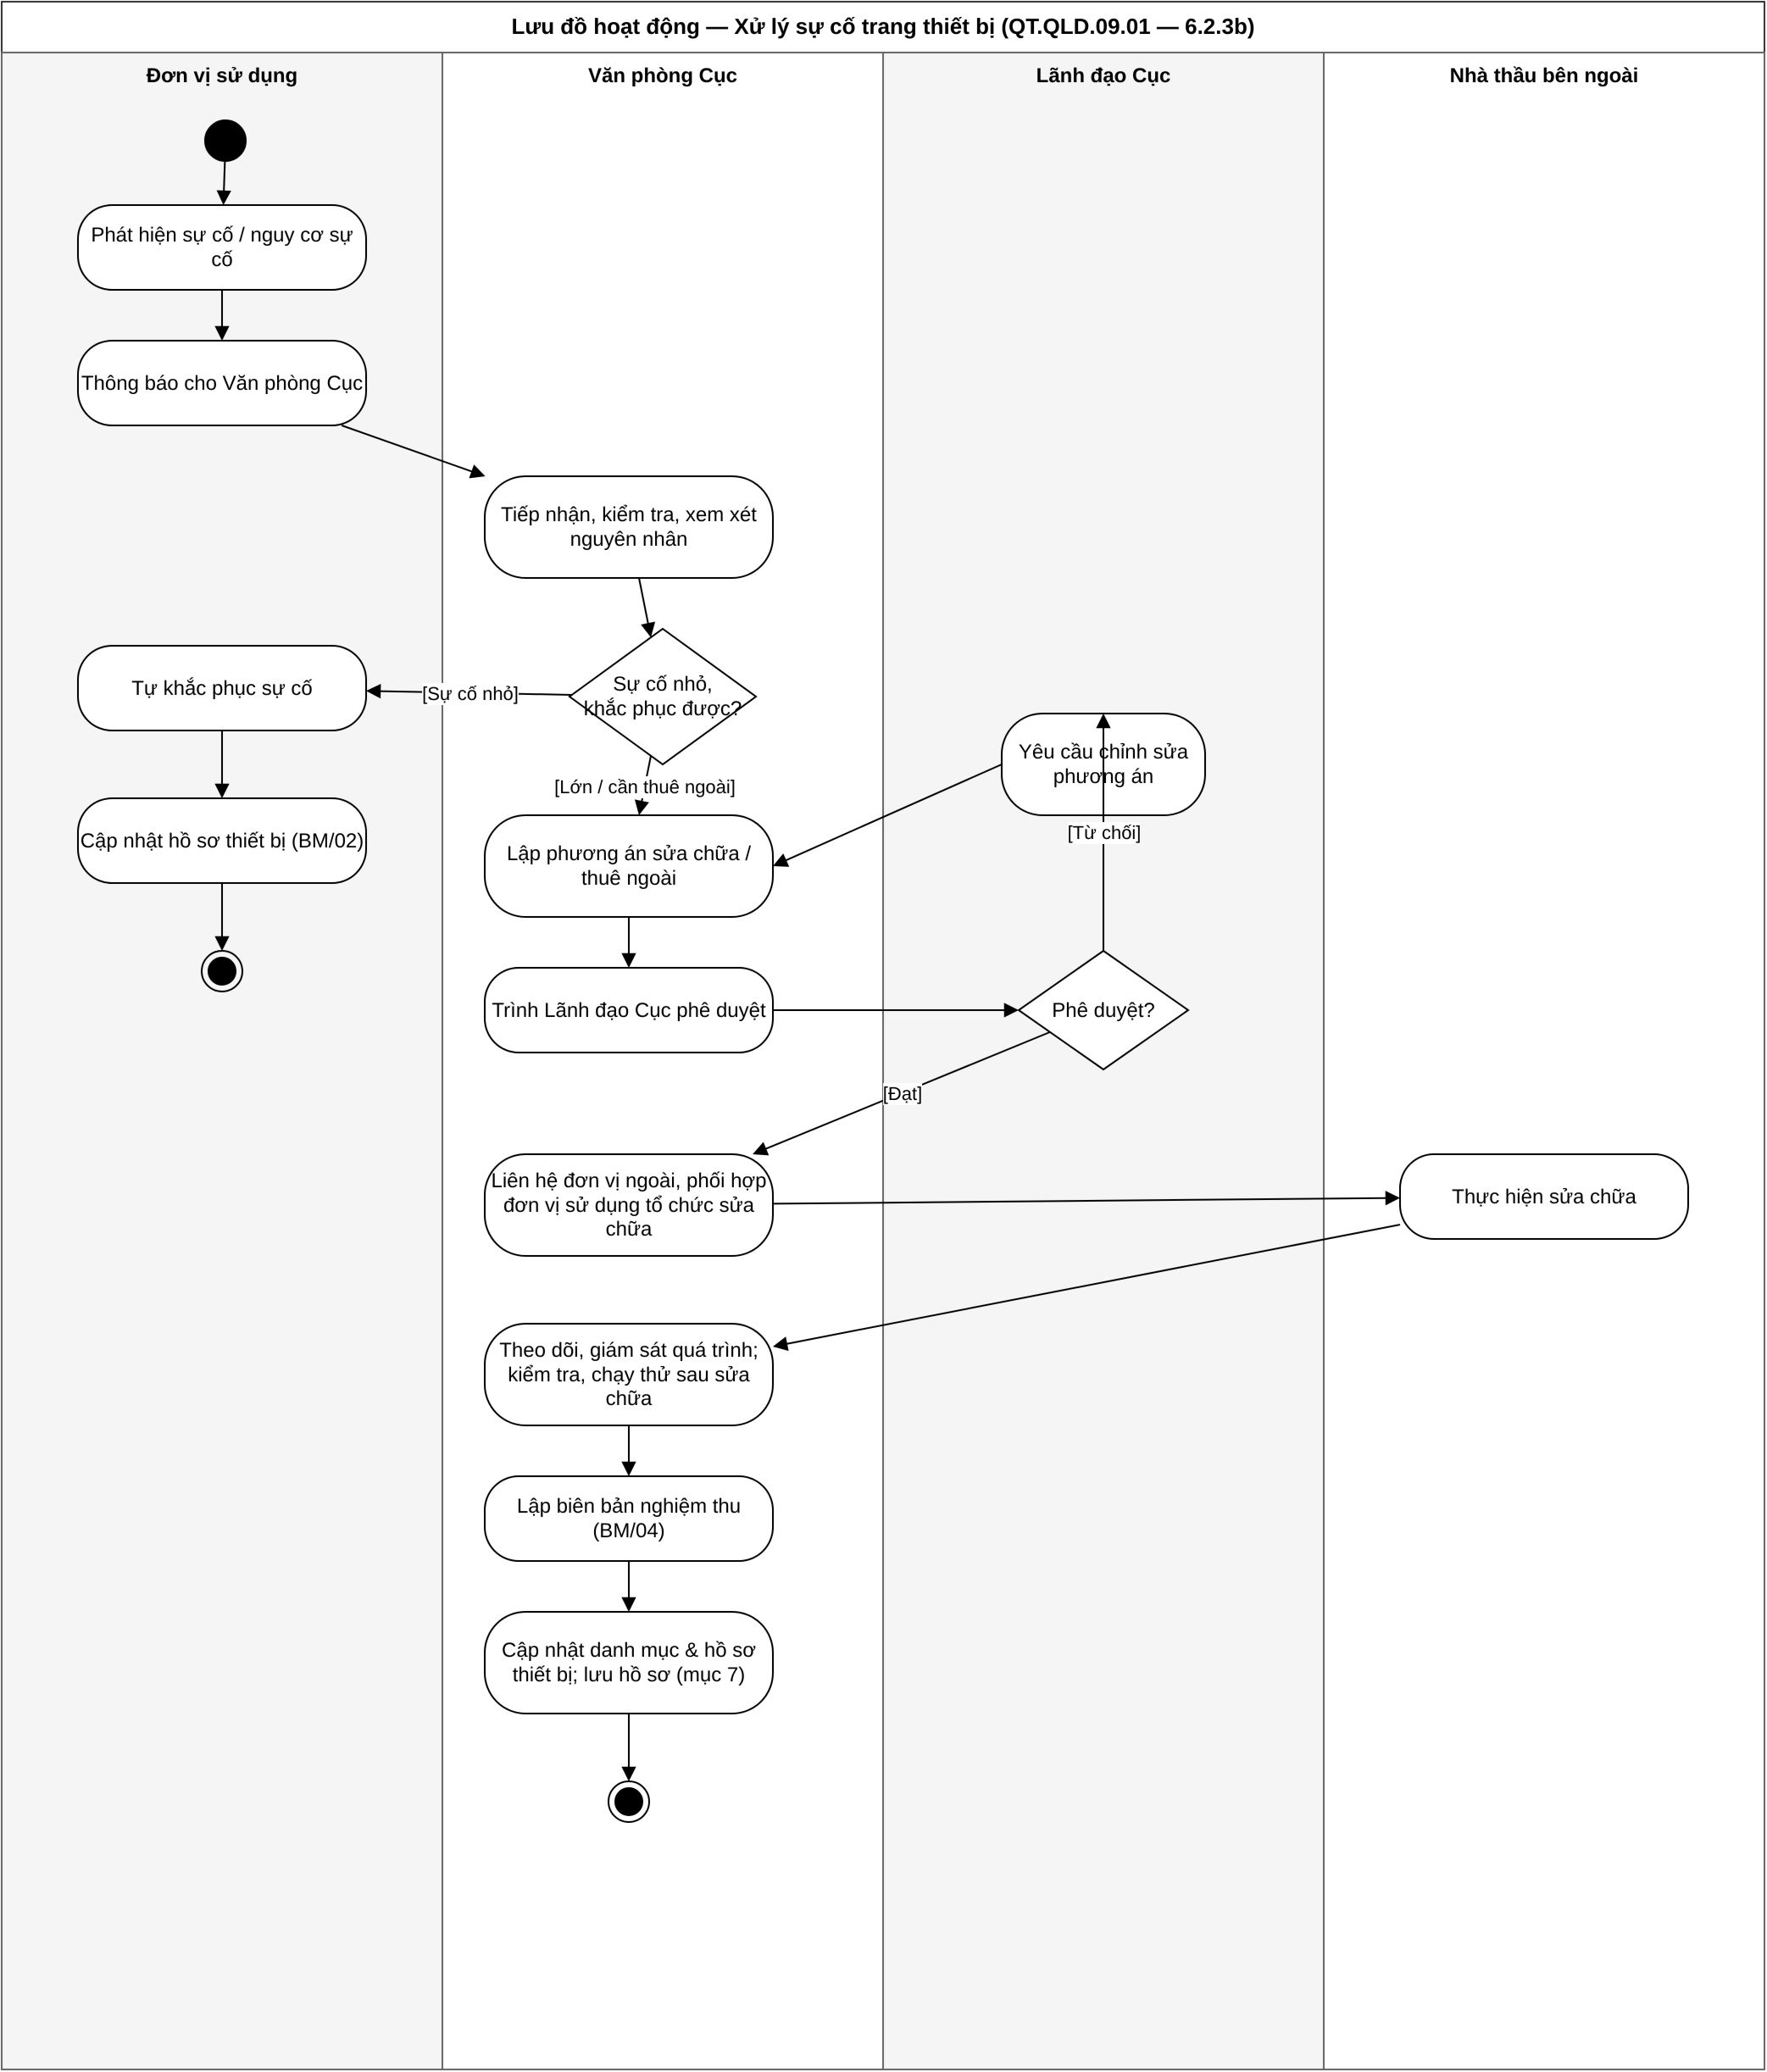
\includegraphics[width=0.86\textwidth]{figures/activity-incident.png}}{\fbox{\parbox{0.9\textwidth}{\centering Sơ đồ hoạt động xử lý sự cố (file \texttt{docs/diagrams/02-activity.drawio}, trang 1)}}}
\caption{Sơ đồ hoạt động — xử lý sự cố (4 phân làn: Đơn vị, Văn phòng Cục, Lãnh đạo Cục, Nhà thầu)}
\label{fig:act-incident}
\end{figure}

Sơ đồ Hình~\ref{fig:act-incident} thể hiện đúng điểm quyết định của mục 6.2.3b: sau khi Văn phòng Cục ``kiểm tra, xem xét nguyên nhân'', nhánh \textbf{[Sự cố nhỏ]} đi thẳng sang làn Đơn vị (tự khắc phục $\rightarrow$ cập nhật hồ sơ $\rightarrow$ kết thúc); nhánh \textbf{[Lớn/cần thuê ngoài]} phải qua làn Lãnh đạo Cục (phê duyệt), nếu bị từ chối quay lại lập lại phương án.

\begin{figure}[h]
\centering
\IfFileExists{figures/activity-plan.png}{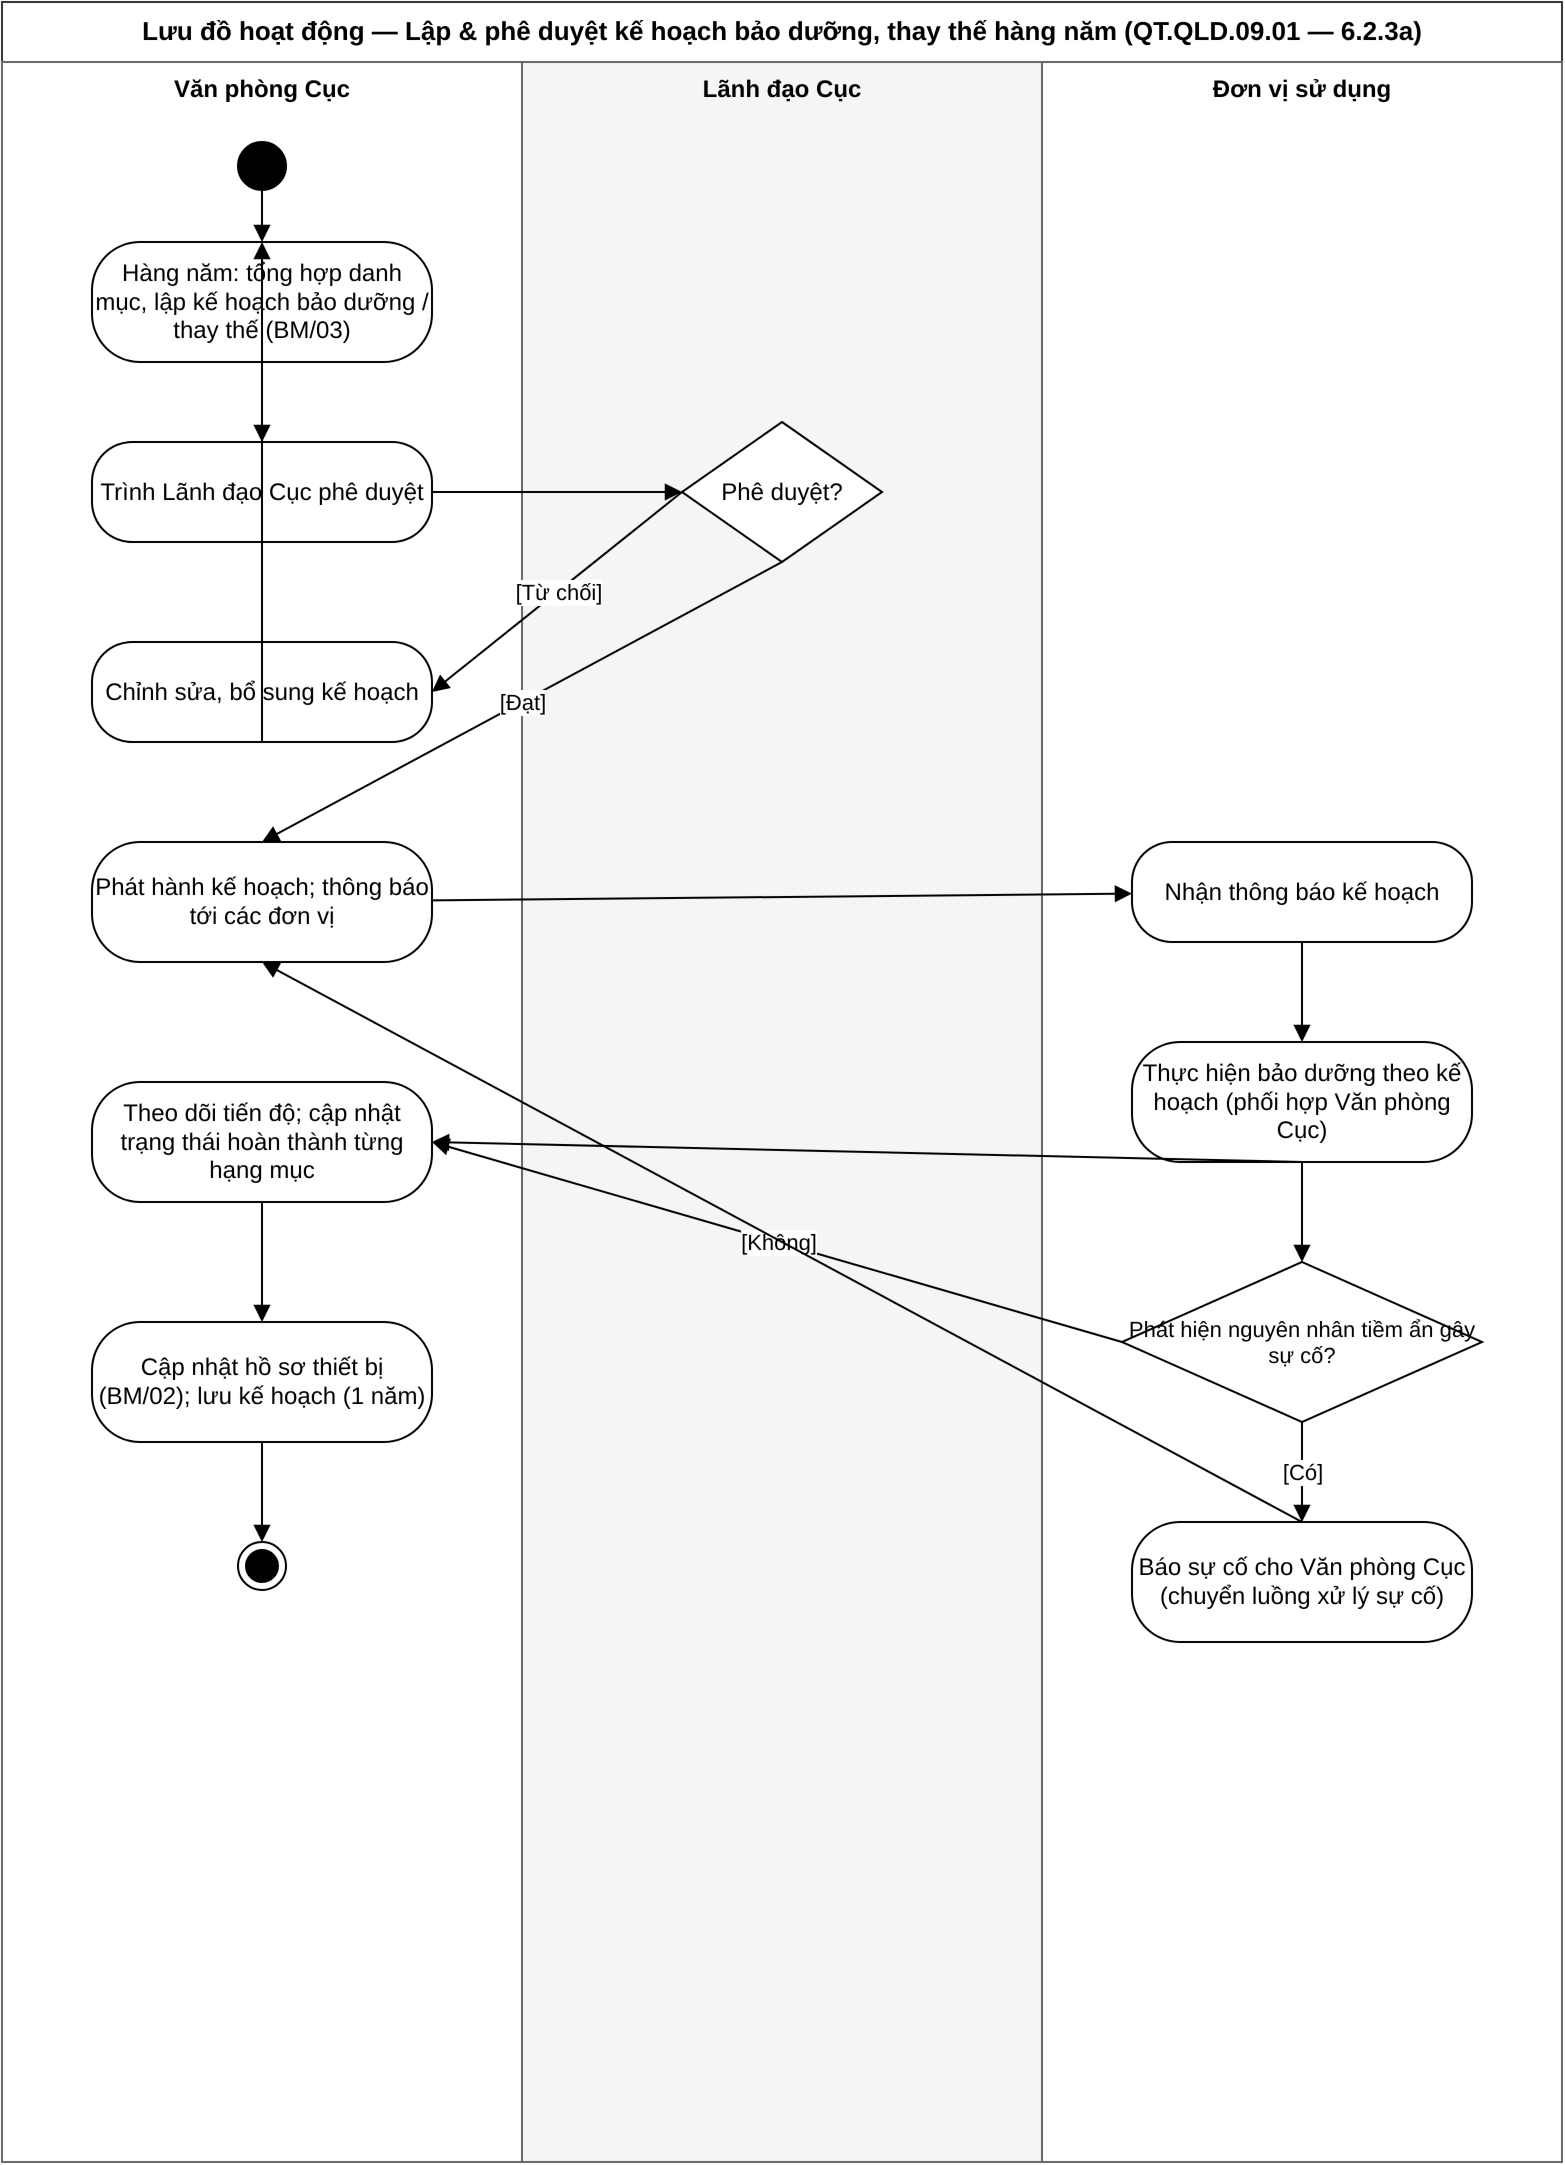
\includegraphics[width=0.8\textwidth]{figures/activity-plan.png}}{\fbox{\parbox{0.9\textwidth}{\centering Sơ đồ hoạt động kế hoạch bảo dưỡng (file \texttt{docs/diagrams/02-activity.drawio}, trang 2)}}}
\caption{Sơ đồ hoạt động — lập và phê duyệt kế hoạch bảo dưỡng hàng năm}
\label{fig:act-plan}
\end{figure}

Sơ đồ Hình~\ref{fig:act-plan} mô tả luồng kế hoạch hàng năm: vòng lặp ``từ chối — chỉnh sửa'' giữa Văn phòng Cục và Lãnh đạo Cục, sau khi phát hành thì các đơn vị thực hiện; nếu phát hiện nguyên nhân tiềm tàng gây sự cố thì chuyển sang luồng xử lý sự cố (mục 6.2.4).
